\documentclass{article}
\usepackage[top=2.5cm, left=3cm, right=3cm, bottom=2.5cm]{geometry}
\usepackage[utf8]{inputenc}
\usepackage{alphabeta}
\usepackage{fullpage}
\usepackage{amsmath,amssymb}
\usepackage{tikz}
\usepackage{listings}
\usepackage{graphicx}
\usepackage{float}
\usepackage{subcaption}

\linespread{1.15}
\title{Image Rectification Toolkit - CV 2025}
\author{Marios Giannopoulos\\Student ID: 1115202000032}
\date{2026-01-06}

\begin{document}
\maketitle
\tableofcontents

\section{Introduction}
\label{sec:introduction}

This toolkit implements a comprehensive image analysis and processing system aimed at rectifying flat rectangular objects from photographs. Rectification is a fundamental task in computer vision that allows the restoration of an object's orthogonal projection from a perspective projection, thereby facilitating further analysis and measurement.

The tool is directly connected to the core topics of the Computer Vision course, as it implements:

\begin{itemize}
    \item \textbf{Convolution and filtering}: Basic image processing techniques for denoising through smoothing and blurring, using mean and Gaussian filters.
    \item \textbf{Edge detection}: Implementation of the Canny algorithm for edge detection, which serves as the foundation for corner detection.
    \item \textbf{Corner detection}: Implementation of the Moravec and Harris algorithms for corner detection, with multi-scale analysis capability.
    \item \textbf{Rectification}: Use of homography for projective transformation of images and restoration of orthogonal projection.
\end{itemize}

All core implementations use exclusively NumPy, while OpenCV is used only for image I/O, color space conversions, and geometric transformations (as allowed by the assignment rules).

\section{Implementation Description}
\label{sec:implementation}

\subsection{Convolution and Filtering}

The basic convolution operation was implemented from scratch, supporting three padding modes: zero, replicate, and reflect. Convolution supports both grayscale and color images, processing each channel separately.

For denoising, two types of filters were implemented:
\begin{itemize}
    \item \textbf{Mean filter}: A simple box filter that computes the average of values in a window, effective for Gaussian noise but causes blurring.
    \item \textbf{Gaussian filter}: A filter that uses a Gaussian kernel, providing better smoothing while preserving more details.
\end{itemize}

For filter evaluation, three noise models were implemented:
\begin{itemize}
    \item \textbf{Gaussian noise}: Additive Gaussian noise with adjustable mean and standard deviation.
    \item \textbf{Impulse noise}: Salt-and-pepper noise that causes random white and black pixels.
    \item \textbf{Poisson noise}: Photon-dependent noise that simulates the photographic process.
\end{itemize}

For color images, two approaches were explored: filtering per RGB channel and filtering only the luminance channel in HSV space.

\subsection{Edge Detection - Canny}

Edge detection was implemented through the Canny algorithm, which consists of five basic steps:

\begin{enumerate}
    \item \textbf{Gaussian smoothing}: Noise reduction before gradient computation.
    \item \textbf{Gradient computation}: Use of Sobel kernels to compute gradients Gx and Gy, and subsequently the magnitude and direction.
    \item \textbf{Non-maximum suppression (NMS)}: Thins edges by keeping only local maxima in the gradient direction.
    \item \textbf{Double thresholding}: Classification of pixels into strong edges, weak edges, and non-edges.
    \item \textbf{Hysteresis thresholding}: Connection of weak edges to strong ones through 8-connected neighborhood.
\end{enumerate}

The implementation allows adjustment of parameters σ (Gaussian smoothing), low threshold, and high threshold, providing flexibility for different image types.

\subsection{Corner Detection}

Two corner detection algorithms were implemented:

\subsubsection{Moravec Corner Detector}
The Moravec algorithm measures intensity variation in different directions around each pixel. A corner is detected when there is significant variation in all directions. The algorithm is simple but less robust than Harris.

\subsubsection{Harris Corner Detector}
The Harris algorithm is more robust and uses the structure tensor (second moment matrix) for corner detection. It computes the product of derivatives (Ixx, Iyy, Ixy), applies Gaussian weighting, and calculates the Harris response as:
\[
R = \det(M) - k \cdot \text{trace}(M)^2
\]
where M is the structure tensor and k is a sensitivity parameter.

For corner selection, 2D non-maximum suppression is applied that selects only local maxima.

\subsubsection{Multi-Scale Analysis}
A Gaussian scale pyramid was implemented that creates multiple versions of the image at different scales, with each level created through smoothing and downsampling by a factor of 2. Corner detection is applied at each level, allowing corner detection at different scales.

\subsection{Rectification}

Rectification is implemented through projective transformation using homography. The process consists of:

\begin{enumerate}
    \item \textbf{Corner detection}: Use of the Harris detector to detect all corners.
    \item \textbf{Selection of 4 corners}: Two methods:
    \begin{itemize}
        \item \textbf{Geometric method}: Selection of corners near the four corners of the image.
        \item \textbf{ROI method}: Selection of the strongest corners within a region of interest.
    \end{itemize}
    \item \textbf{Corner ordering}: Organization of the 4 corners as [top-left, top-right, bottom-left, bottom-right].
    \item \textbf{Homography computation}: Use of the \texttt{cv2.getPerspectiveTransform} function (allowed) to compute the homography matrix.
    \item \textbf{Transformation application}: Use of \texttt{cv2.warpPerspective} (allowed) to apply the projective transformation.
\end{enumerate}

The size of the rectified image is automatically calculated based on the distances between the selected corners.

\section{Results}
\label{sec:results}

\subsection{Denoising}

\begin{figure}[H]
    \centering
    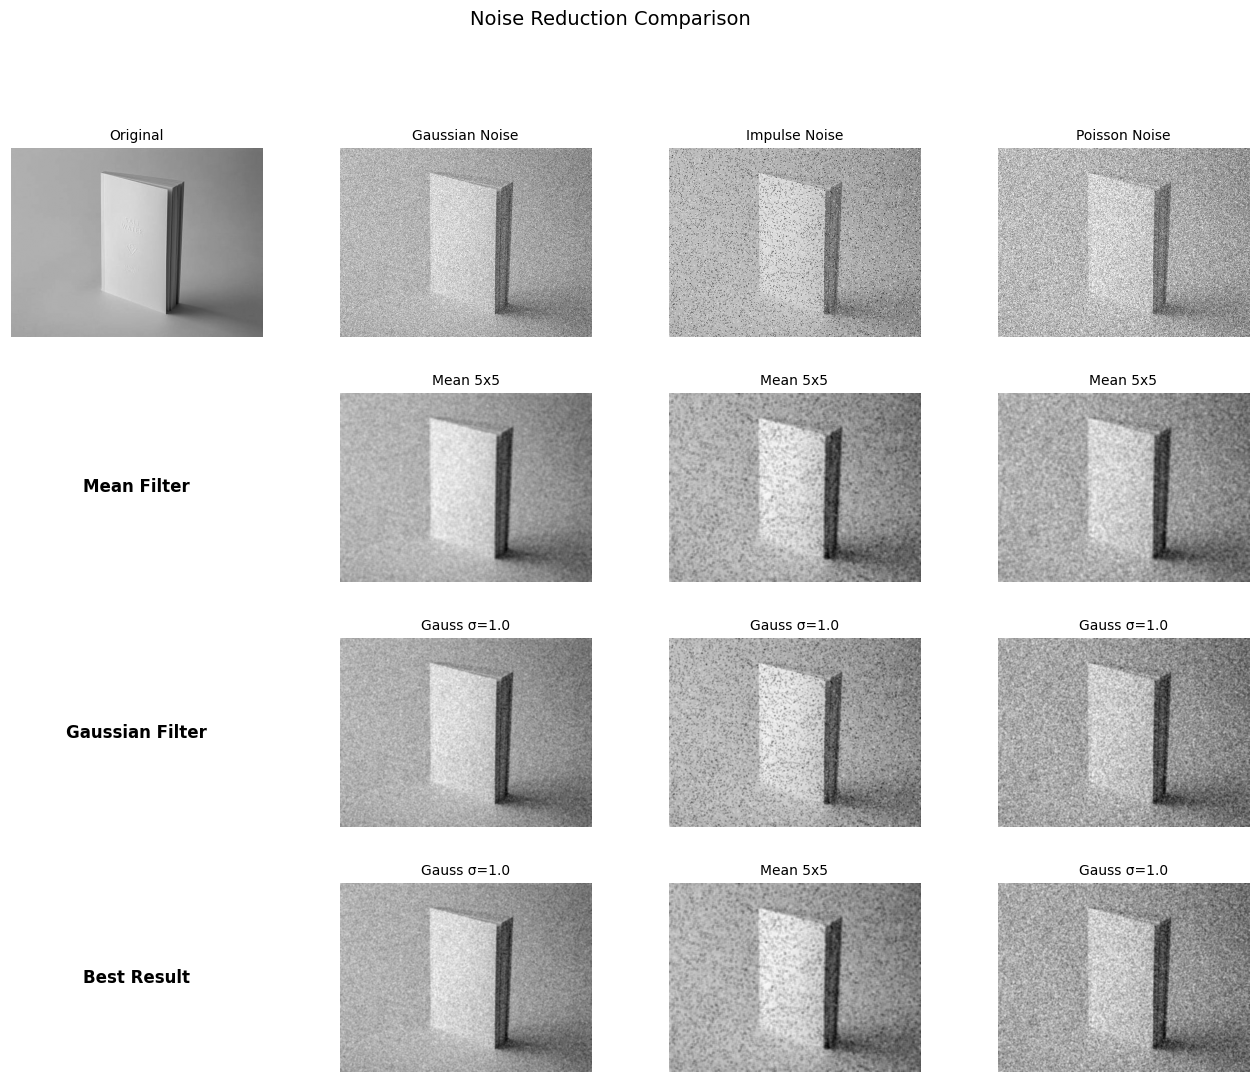
\includegraphics[width=0.8\textwidth]{assets/noisy_and_filtered.png}
    \caption{Comparison of original, noisy (Gaussian, impulse, Poisson) and filtered images}
    \label{fig:noisy_and_filtered}
\end{figure}

Experimental tests showed that:

\textbf{Gaussian noise}: The Gaussian filter with σ=1.0 showed the best performance, effectively restoring the image with minimal loss of details. The mean filter (5x5) was also effective but caused more blurring, especially at edges.

\textbf{Impulse noise}: The mean filter was more effective than Gaussian for salt-and-pepper noise, as averaging helps eliminate isolated outlier pixels. However, both filters had difficulties with high noise levels (>10\%).

\textbf{Poisson noise}: The Gaussian filter with moderate σ (1.0-1.5) provided a good balance between denoising and detail preservation.

\begin{figure}[H]
    \centering
    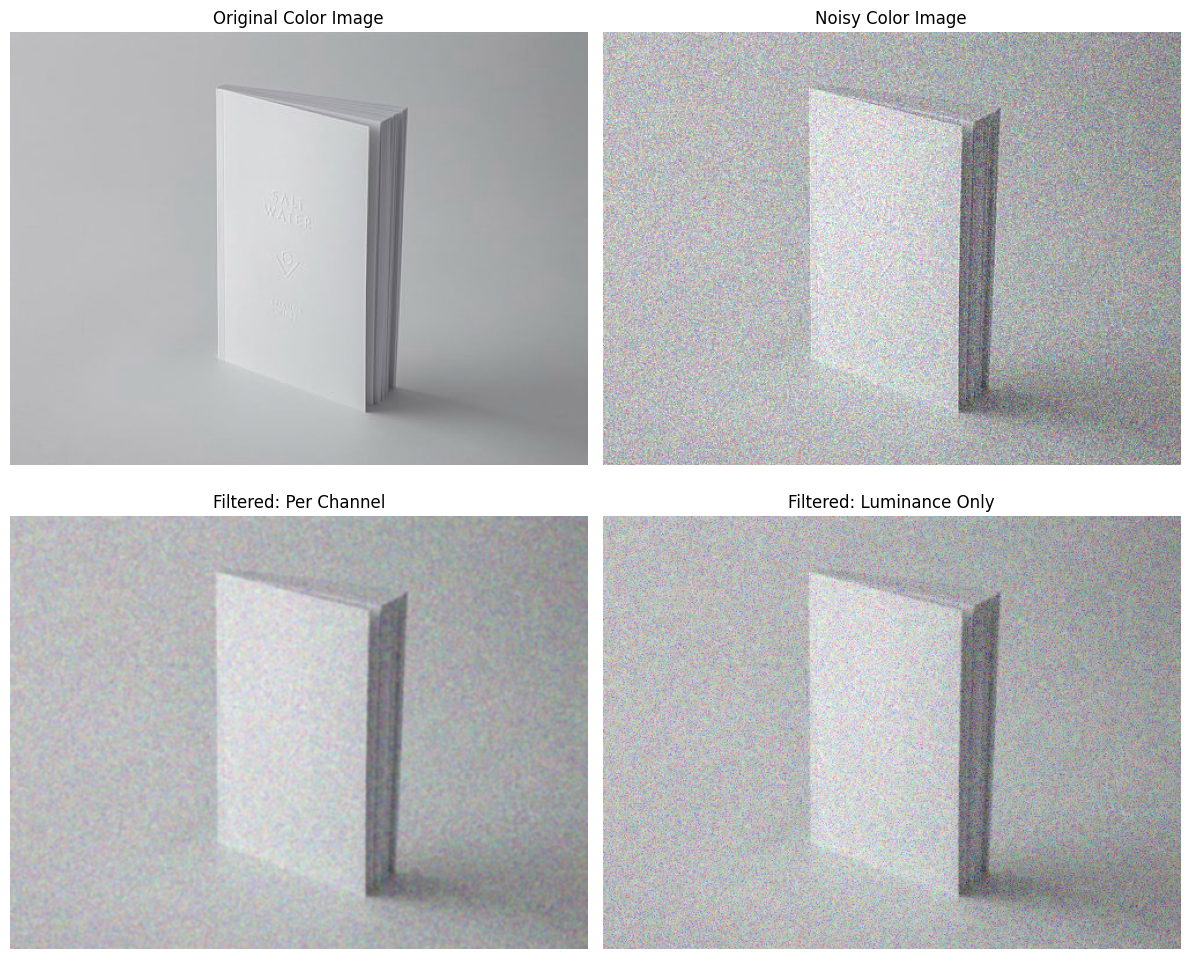
\includegraphics[width=0.8\textwidth]{assets/color_filtering.png}
    \caption{Comparison of color image filtering methods (per-channel vs luminance-only)}
    \label{fig:color_filtering}
\end{figure}

For color images, filtering only the luminance channel (HSV) provided better results, preserving colors while reducing noise, whereas filtering per RGB channel could cause color distortions.

\subsection{Edge Detection}

\begin{figure}[H]
    \centering
    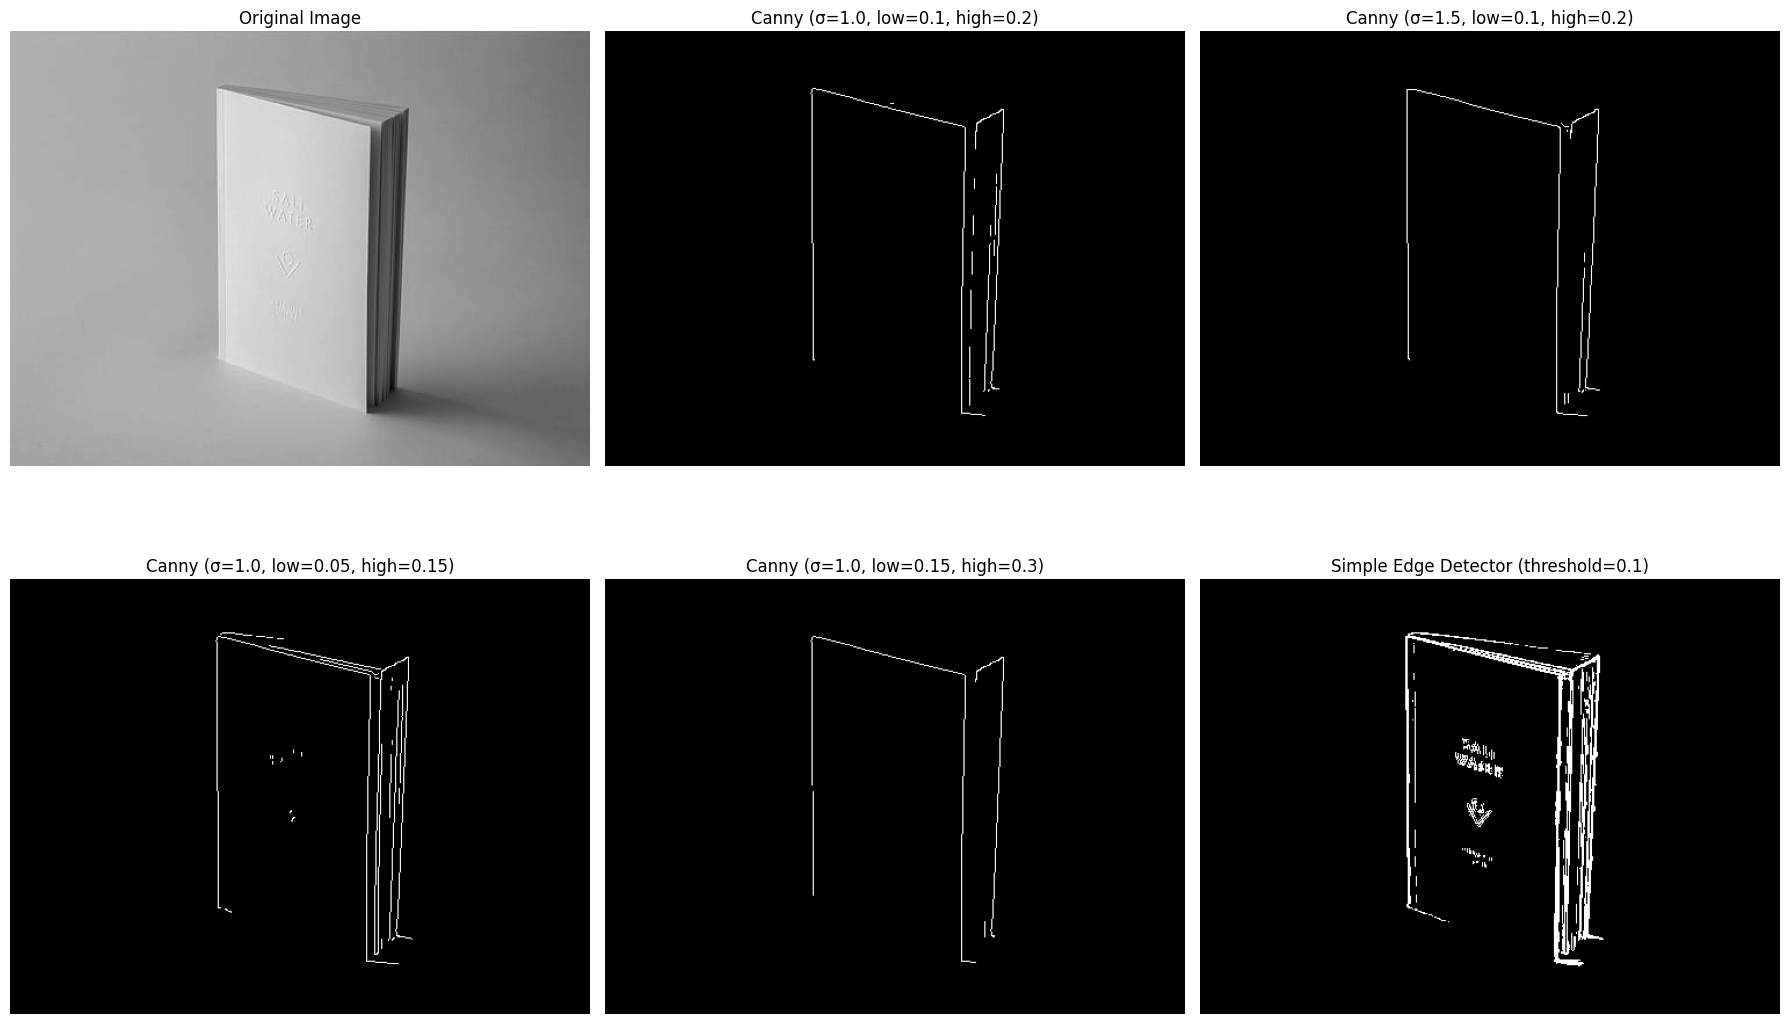
\includegraphics[width=0.8\textwidth]{assets/canny_edge_detection.png}
    \caption{Canny edge detection with varying parameters}
    \label{fig:canny_edge_detection}
\end{figure}

The Canny implementation showed good results. Observations:

\textbf{Successes}:
\begin{itemize}
    \item NMS effectively thins edges, creating single-pixel-thick edges.
    \item Hysteresis thresholding successfully connects weak edges to strong ones, creating continuous edges.
    \item The algorithm is robust to noise when appropriate σ (1.0-1.5) is used.
\end{itemize}

\textbf{Challenges}:
\begin{itemize}
    \item Threshold selection is critical: too low thresholds lead to many false edges, while too high thresholds miss weak edges.
    \item In images with heavy noise, even with smoothing, false edges remain.
    \item Comparison with OpenCV Canny showed that our implementation is more conservative (fewer edges), possibly due to different hysteresis implementation.
\end{itemize}

\begin{figure}[H]
    \centering
    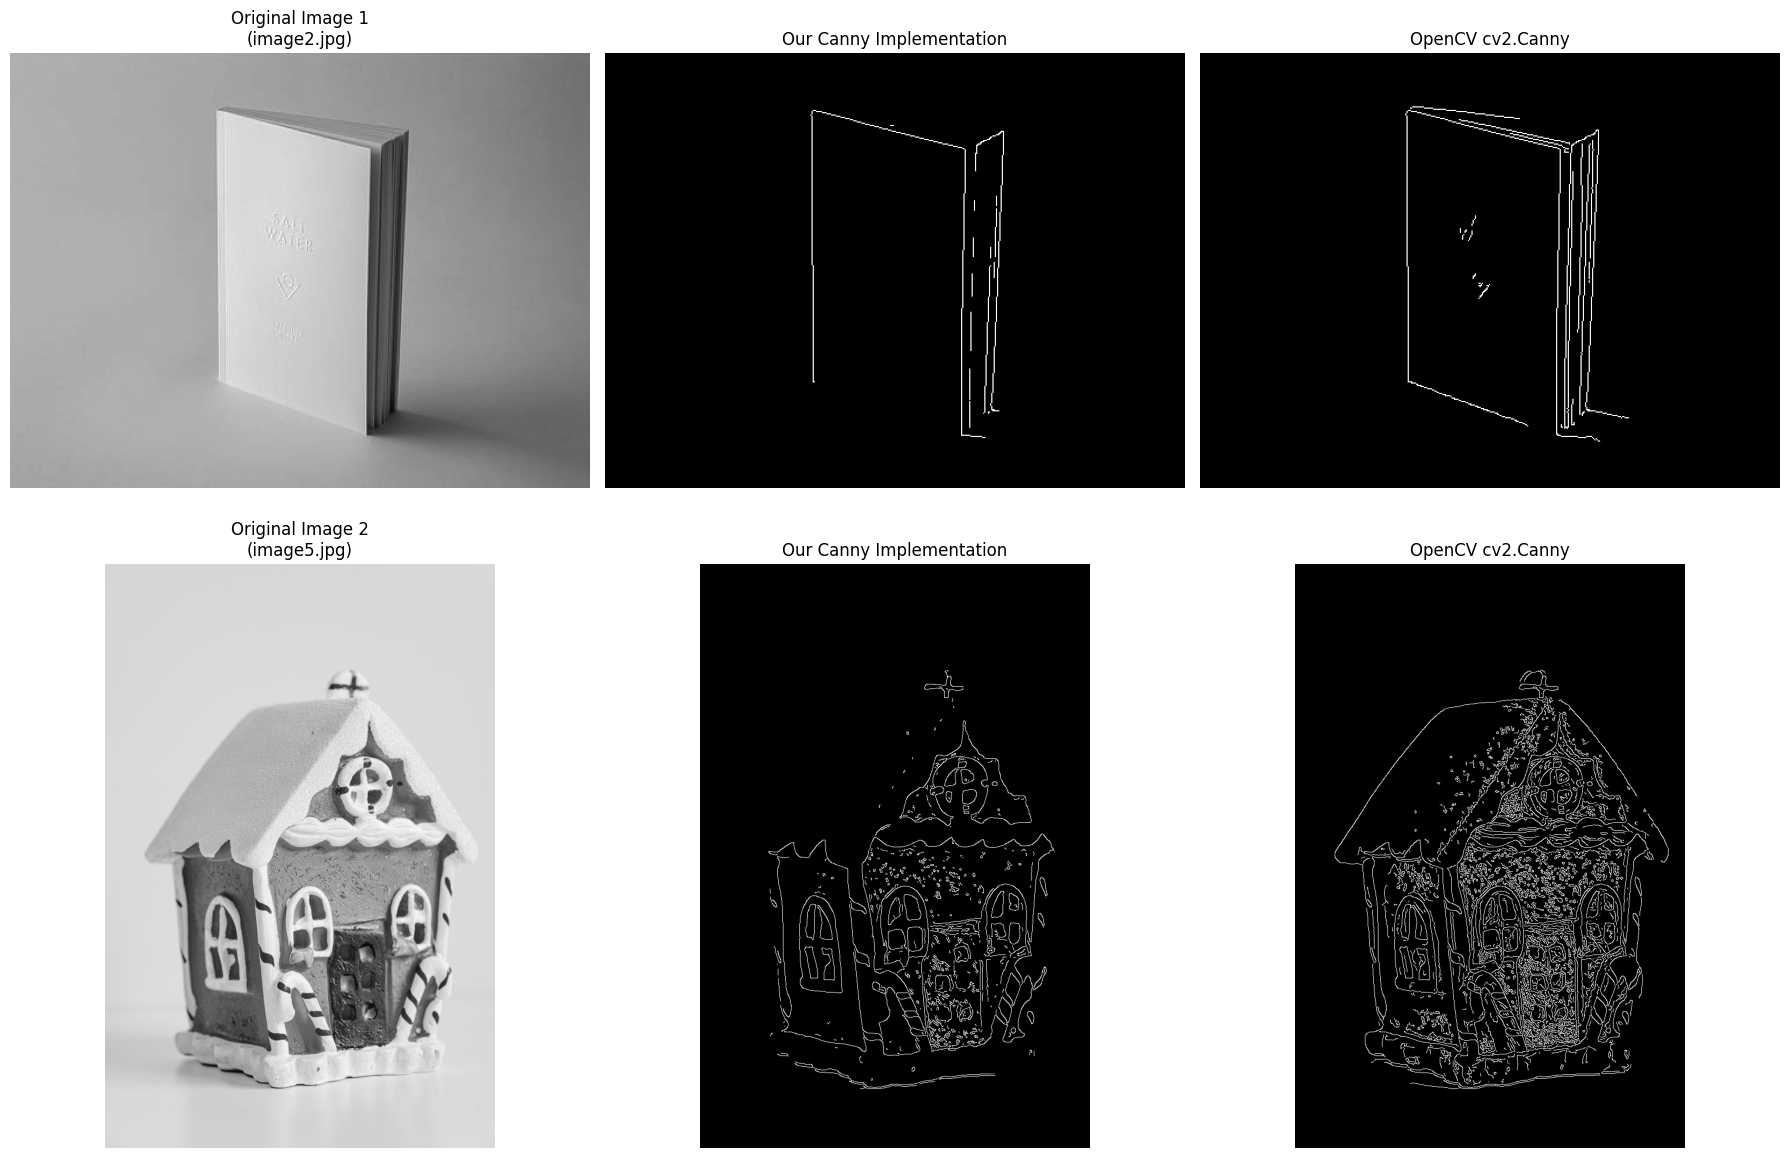
\includegraphics[width=0.8\textwidth]{assets/canny_opencv_comparison.png}
    \caption{Comparison of our Canny implementation with OpenCV Canny}
    \label{fig:canny_opencv_comparison}
\end{figure}

\subsection{Corner Detection}

\begin{figure}[H]
    \centering
    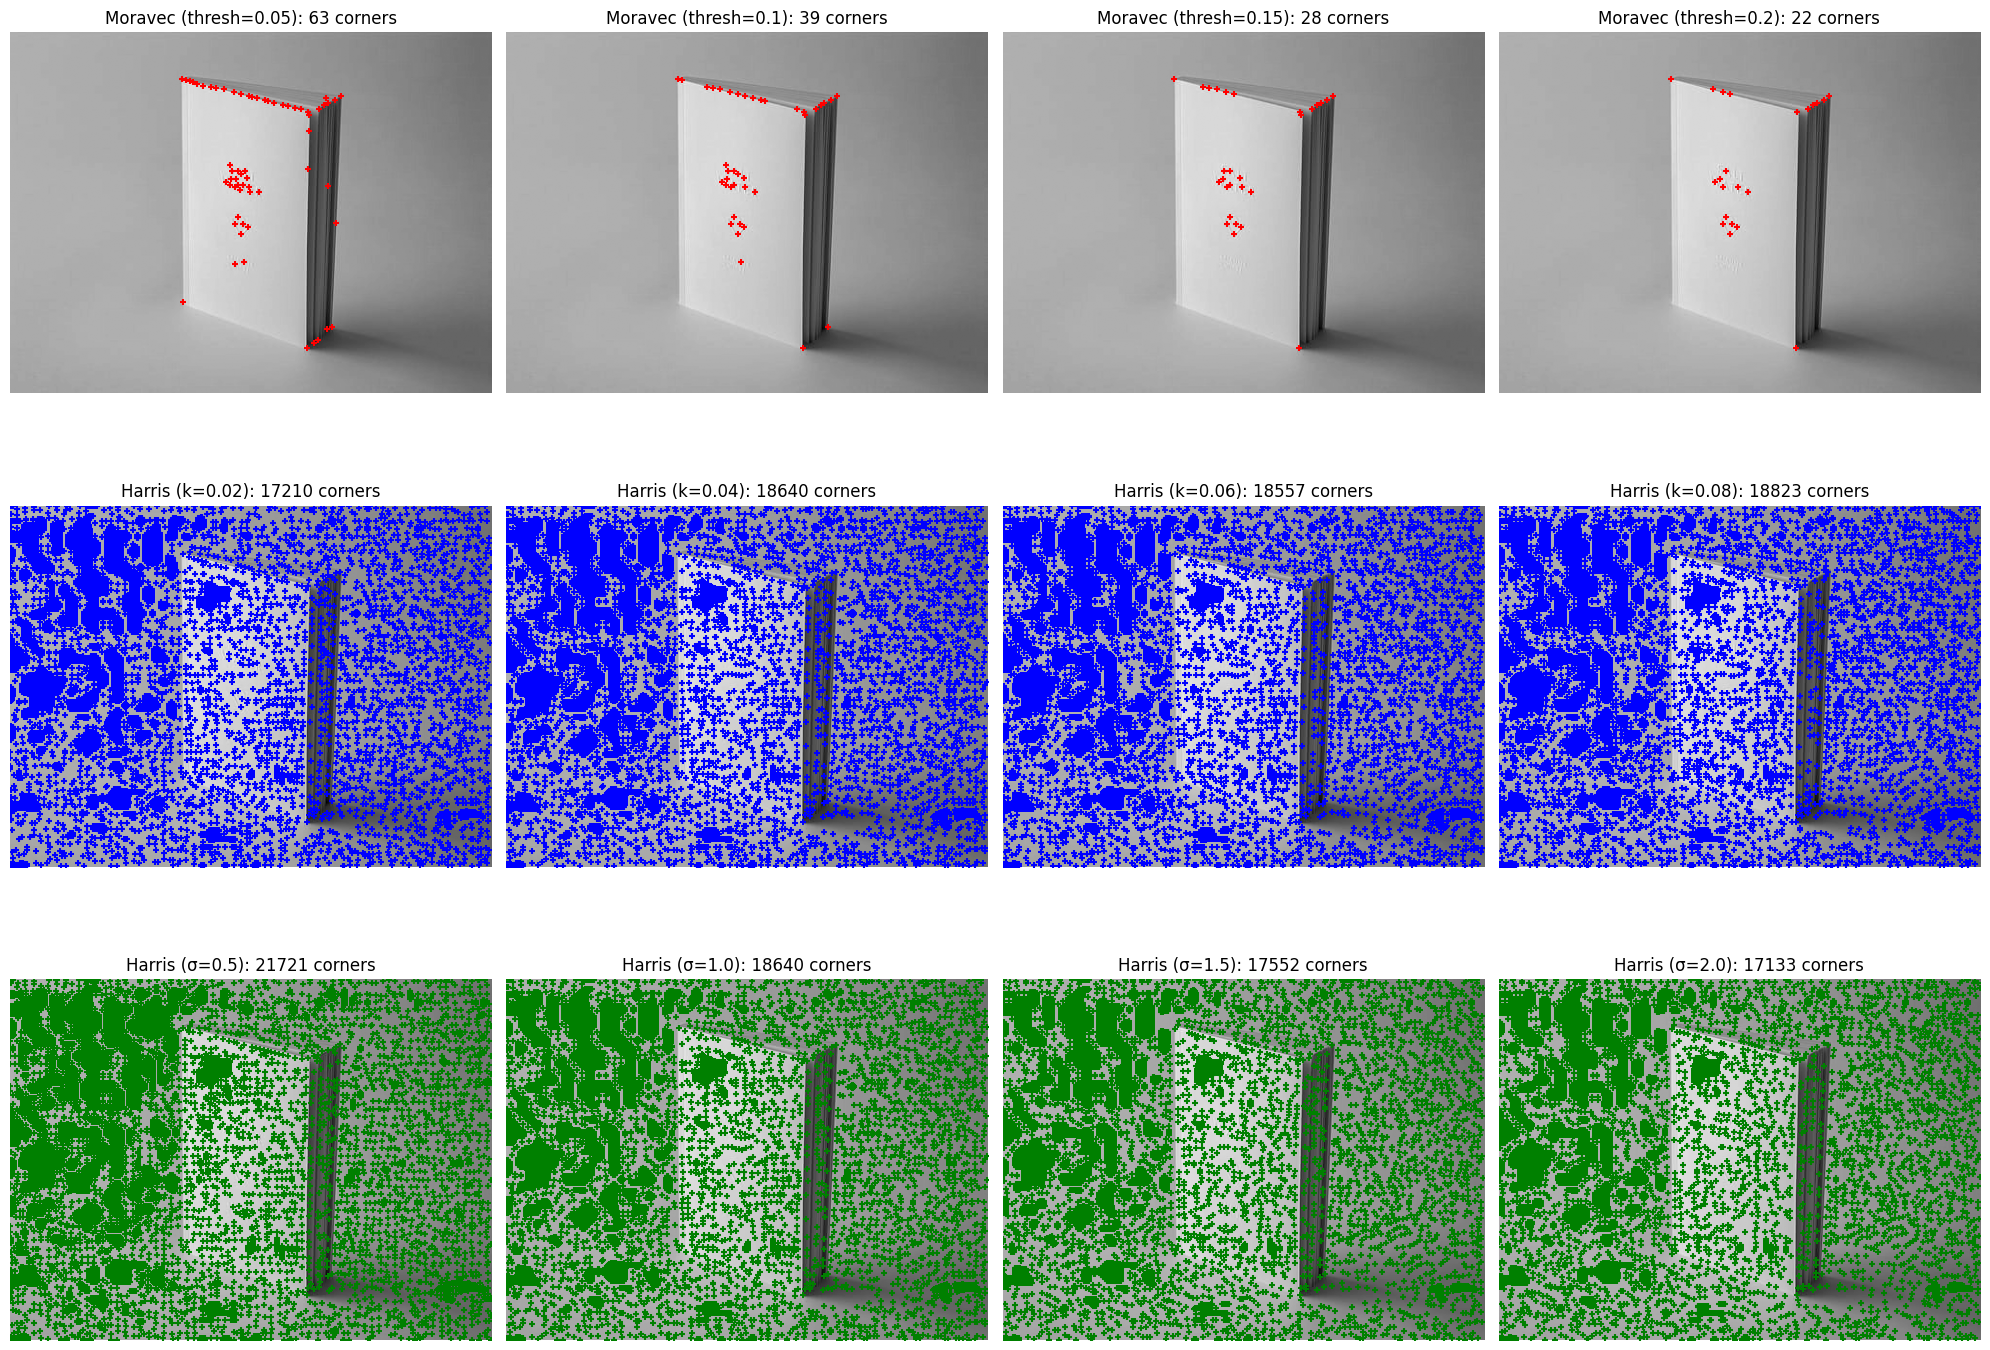
\includegraphics[width=0.8\textwidth]{assets/moravec_harris_comparison.png}
    \caption{Comparison of Moravec and Harris corner detection}
    \label{fig:moravec_harris_comparison}
\end{figure}

\textbf{Moravec Detector}: The Moravec algorithm detected fewer corners (39-214 per image) and was more selective. However, it was more sensitive to noise and less accurate in corner localization.

\textbf{Harris Detector}: The Harris algorithm was much more sensitive, detecting thousands of corners. This requires careful parameter tuning:
\begin{itemize}
    \item \textbf{k parameter}: Smaller values (0.02-0.04) detect more corners, while larger ones (0.06-0.08) are more selective.
    \item \textbf{σ (smoothing)}: Smaller σ (0.5-1.0) detects fine details, while larger (1.5-2.0) provides more stable but fewer corners.
    \item \textbf{NMS threshold}: Critical for controlling the number of corners.
\end{itemize}

% TODO: Add image - Multi-scale corner detection results
% [IMAGE PLACEHOLDER 6: Multi-scale corner detection pyramid and results]

\begin{figure}[H]
    \centering
    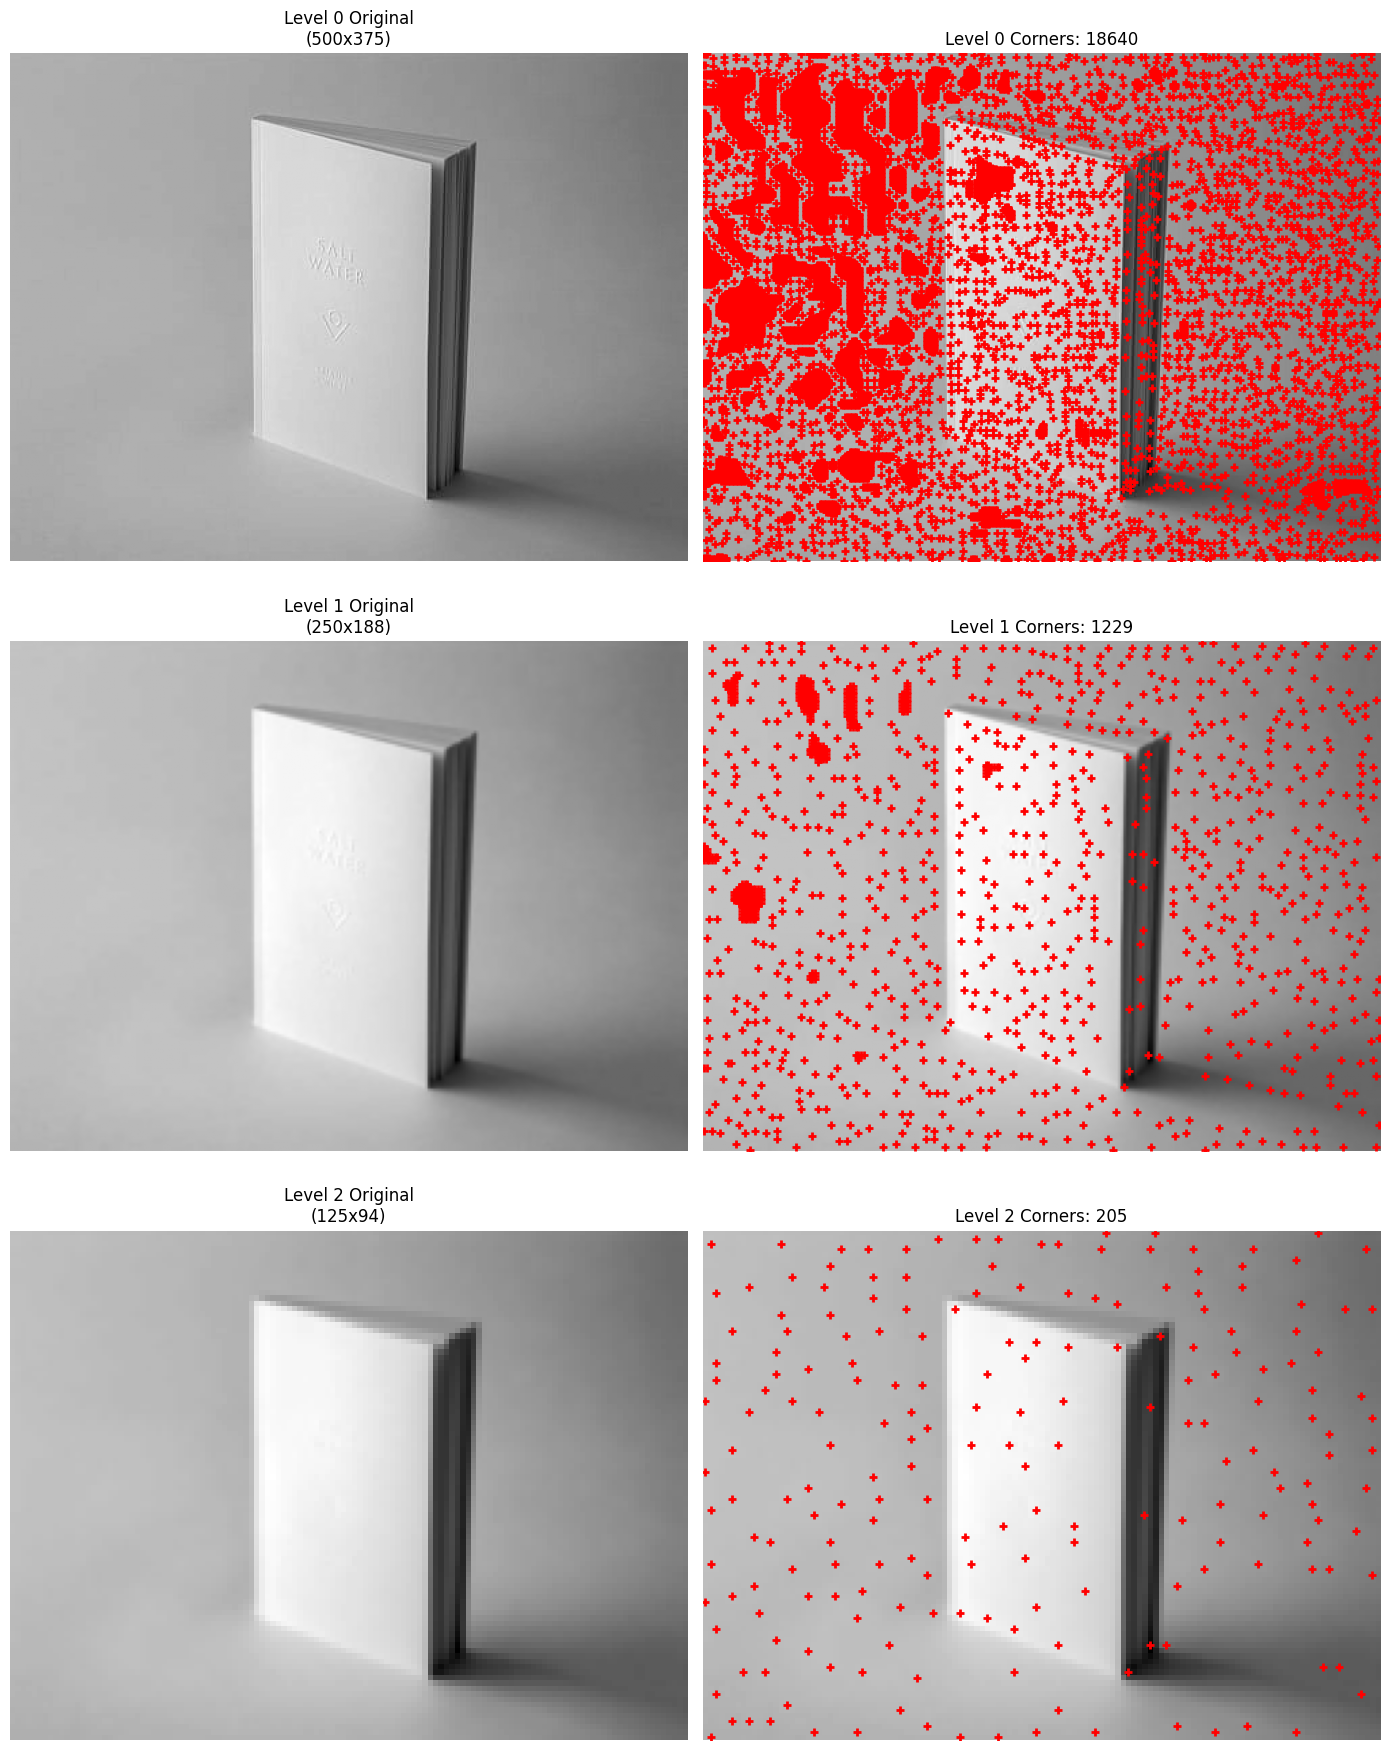
\includegraphics[width=0.8\textwidth]{assets/multi_scale_corner_detection.png}
    \caption{Multi-scale corner detection}
    \label{fig:multi_scale_corner_detection}
\end{figure}

\textbf{Multi-Scale Analysis}: Analysis at different scales showed that:
\begin{itemize}
    \item At level 0 (full size) the most corners are detected (18640 for the first image).
    \item At lower levels (downsampled) fewer but more stable corners are detected (1229 at level 1, 205 at level 2).
    \item Corner density (corners/pixel) decreases at lower levels, indicating that corners are detected at larger structures.
\end{itemize}

\subsection{Rectification}
\begin{figure}[H]
    \centering
    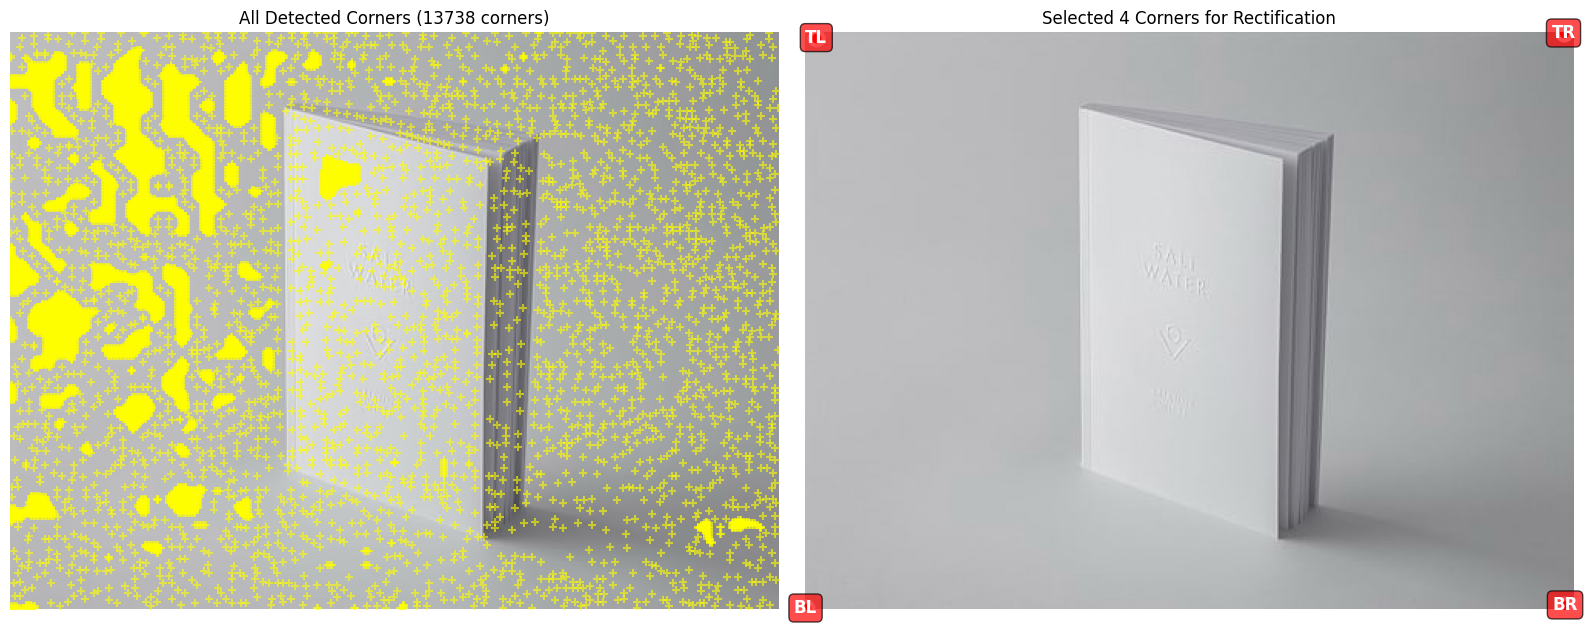
\includegraphics[width=0.8\textwidth]{assets/rectification_comparison.png}
    \caption{Comparison of original and rectified images}
    \label{fig:rectification_comparison}
\end{figure}

The rectification process showed good results when corners were detected correctly:

\textbf{Successes}:
\begin{itemize}
    \item The geometric method for corner selection worked well for images where the rectangular object covers a significant portion of the image.
    \item The calculation of the rectified image size based on distances between corners provided reasonable results.
    \item The projective transformation successfully restored the orthogonal projection.
\end{itemize}

\begin{figure}[H]
    \centering
    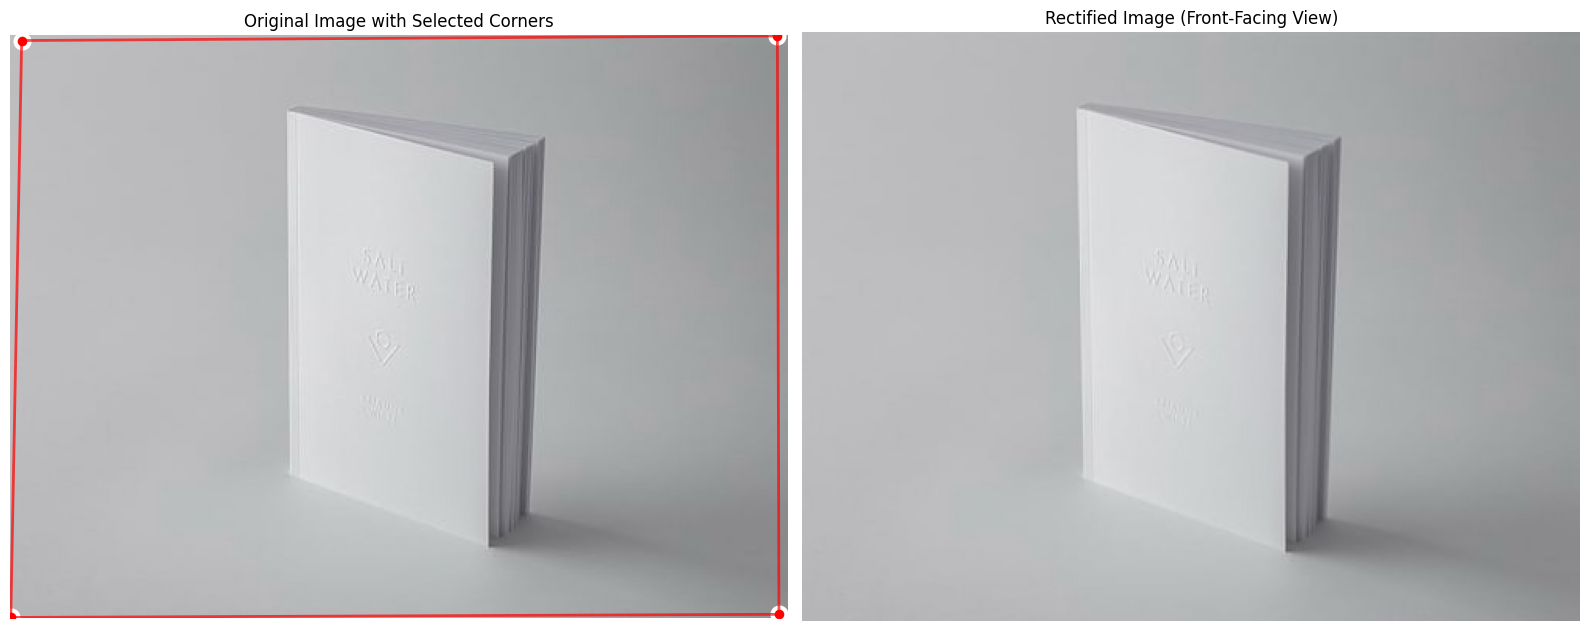
\includegraphics[width=0.8\textwidth]{assets/original_vs_rectified.png}
    \caption{Comparison of original and rectified images}
    \label{fig:original_vs_rectified}
\end{figure}

\textbf{Challenges and Limitations}:
\begin{itemize}
    \item \textbf{Corner selection accuracy}: Automatic selection of 4 corners may choose incorrect corners, especially when there are many corners or when the object is not clearly separated.
    \item \textbf{Sensitivity to errors}: Sensitivity analysis showed that even small corner shifts (±2-5 pixels) can cause visible distortions in the rectified image.
    \item \textbf{Harris parameters}: The high sensitivity of Harris requires careful parameter tuning to select the correct corners.
    \item \textbf{Sub-pixel accuracy}: The implementation does not support sub-pixel refinement, limiting accuracy.
\end{itemize}

\begin{figure}[H]
    \centering
    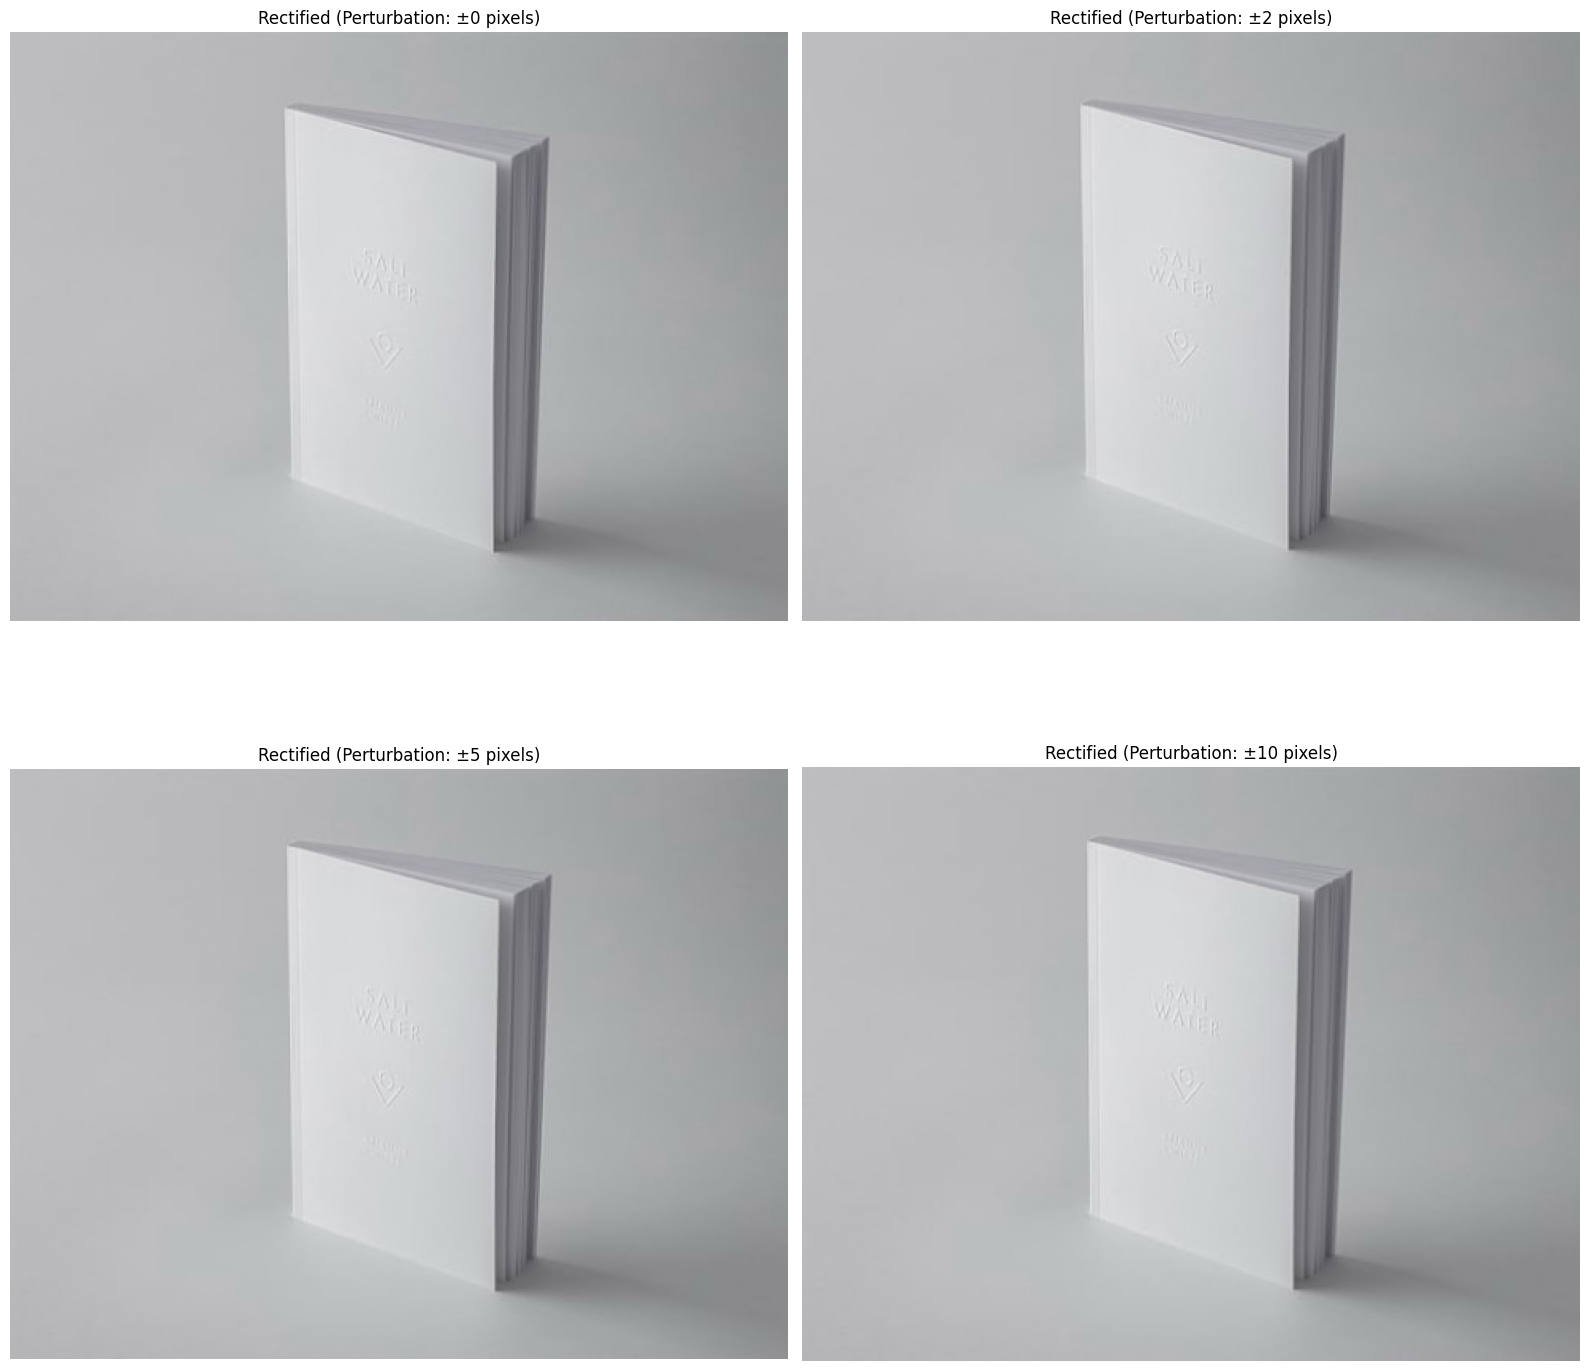
\includegraphics[width=0.8\textwidth]{assets/sensitivity_analysis.png}
    \caption{Sensitivity analysis with different corner perturbations}
    \label{fig:sensitivity_analysis}
\end{figure}

\section{Conclusion}
\label{sec:conclusion}

The implementation of the Image Rectification Toolkit provided deep understanding of fundamental computer vision techniques. The core mathematical concepts (convolution, gradients, structure tensor, homography) were implemented from scratch, allowing full understanding of their operation.

\textbf{Key Lessons}:
\begin{itemize}
    \item Parameter selection is critical for each algorithm and depends on the properties of each image.
    \item Preprocessing (smoothing, noise reduction) is necessary for reliable results in more complex algorithms.
    \item Multi-scale analysis provides more stable and reliable detections.
    \item Automatic feature selection (such as corners) is more difficult than their detection.
\end{itemize}

\textbf{Approach Limitations}:
\begin{itemize}
    \item Automatic selection of 4 corners for rectification is sensitive and may require manual intervention for complex images.
    \item The lack of sub-pixel refinement limits corner detection accuracy.
    \item The implementations, while correct, are not optimized for speed (use of nested loops instead of vectorization in some places).
    \item Corner detection can be difficult in images with heavy noise or low contrast.
\end{itemize}

\textbf{Future Improvements}:
\begin{itemize}
    \item Implementation of sub-pixel corner refinement for greater accuracy.
    \item Interactive corner selection with manual correction capability.
    \item Improvement of corner selection algorithm using geometric constraints (e.g., enforcing rectangle properties).
    \item Performance optimization with vectorization and parallel processing.
    \item Extension for detection and rectification of non-rectangular objects.
\end{itemize}

Overall, the tool achieves its main goal (rectification of rectangular objects) and provides a solid foundation for further development and improvement.

\end{document}